\documentclass[tikz,border=8pt,multi=tikzpicture]{standalone}
\usepackage{amsmath}
\usepackage{xcolor}
\usetikzlibrary{arrows.meta, calc}

\definecolor{mainblue}{HTML}{001158}
\definecolor{accent}{HTML}{8592bc}
\definecolor{lightaccent}{HTML}{e7e9f2}

\tikzset{
  force/.style={-{Stealth[length=3mm]}, line width=1.2pt, color=mainblue},
  dim/.style={-{Stealth[length=2mm]}, line width=0.7pt, color=accent},
  moment/.style={-{Stealth[length=2.5mm]}, line width=1.2pt, color=mainblue},
  qload/.style={-{Stealth[length=2mm]}, line width=0.9pt, color=mainblue!70},
  every node/.append style={font=\sffamily}
}

\newcommand{\festlager}[1]{
  \begin{scope}[shift={#1}]
    \draw[line width=1pt] (0,0) -- (-0.3,-0.5) -- (0.3,-0.5) -- cycle;
    \draw[line width=1pt] (-0.42,-0.5) -- (0.42,-0.5);
    \foreach \x in {-0.42,-0.24,...,0.42} {\draw[line width=0.4pt] (\x,-0.5) -- (\x-0.13,-0.68);}
  \end{scope}
}
\newcommand{\loslager}[1]{
  \begin{scope}[shift={#1}]
    \draw[line width=1pt] (0,0) -- (-0.3,-0.5) -- (0.3,-0.5) -- cycle;
    \foreach \x in {-0.18,0,0.18} {\draw[fill=white, line width=0.7pt] (\x,-0.6) circle (0.1);}
    \draw[line width=1pt] (-0.42,-0.72) -- (0.42,-0.72);
    \foreach \x in {-0.42,-0.24,...,0.42} {\draw[line width=0.4pt] (\x,-0.72) -- (\x-0.13,-0.9);}
  \end{scope}
}
\newcommand{\einspannung}[1]{
  \begin{scope}[shift={#1}]
    \draw[mainblue, line width=1.5pt] (0,0.6) -- (0,-0.6);
    \foreach \y in {-0.5,-0.25,...,0.5} {\draw[line width=0.5pt] (0,\y) -- (-0.25,\y+0.22);}
  \end{scope}
}
\newcommand{\gelenk}[1]{
  \begin{scope}[shift={#1}]
    \draw[draw=mainblue, fill=white, line width=1.3pt] (0,0) circle (0.13);
  \end{scope}
}
\newcommand{\pendelstuetze}[1]{
  % pin support via a 45-degree strut hanging below the beam point #1
  \begin{scope}[shift={#1}]
    \draw[fill=white, line width=0.8pt] (0,0) circle (0.08);
    \draw[line width=1.4pt] (0,0) -- (0.9,-1.55);
    \draw[fill=white, line width=0.8pt] (0.9,-1.55) circle (0.08);
    \draw[line width=1pt] (0.5,-1.75) -- (1.3,-1.75);
    \foreach \x in {0.5,0.7,...,1.3} {\draw[line width=0.4pt] (\x,-1.75) -- (\x-0.13,-1.93);}
  \end{scope}
}

\begin{document}

% ================= Ex 8.1 problem: fixed + hinge + Pendelstuetze + overhang =================
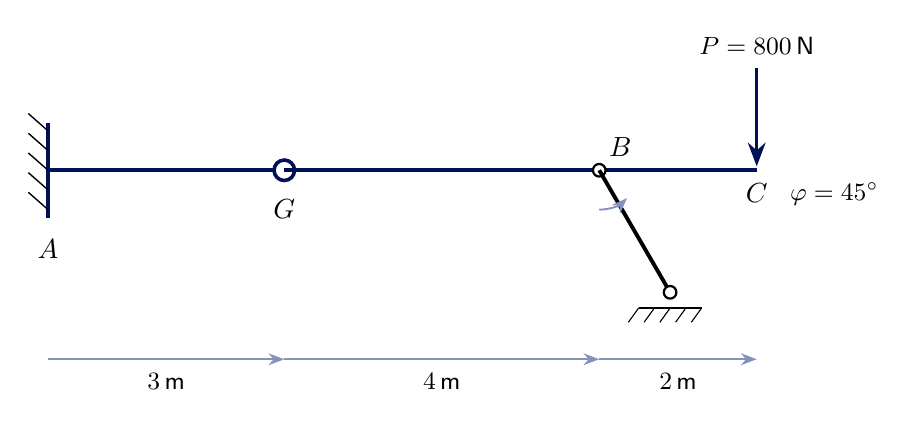
\begin{tikzpicture}
\einspannung{(0,0)}
\draw[mainblue, line width=1.5pt] (0,0) -- (3,0);
\gelenk{(3,0)}
\draw[mainblue, line width=1.5pt] (3,0) -- (9,0);
\pendelstuetze{(7,0)}
\node[below] at (0,-0.75) {$A$};
\node[below] at (3,-0.25) {$G$};
\node[above right] at (7,0.05) {$B$};
\node[right] at (9.3,-0.3) {\small $\varphi=45^\circ$};
\draw[dim] (7,-0.5) arc (270:315:0.5);
\node[below] at (9,-0.05) {$C$};
\draw[force] (9,1.3) -- (9,0.05);
\node[above] at (9,1.35) {\small $P=800\,\text{N}$};
\draw[dim] (0,-2.4) -- (3,-2.4);
\node[below] at (1.5,-2.45) {\small $3\,\text{m}$};
\draw[dim] (3,-2.4) -- (7,-2.4);
\node[below] at (5,-2.45) {\small $4\,\text{m}$};
\draw[dim] (7,-2.4) -- (9,-2.4);
\node[below] at (8,-2.45) {\small $2\,\text{m}$};
\end{tikzpicture}

% ================= Ex 8.1 split free bodies =================
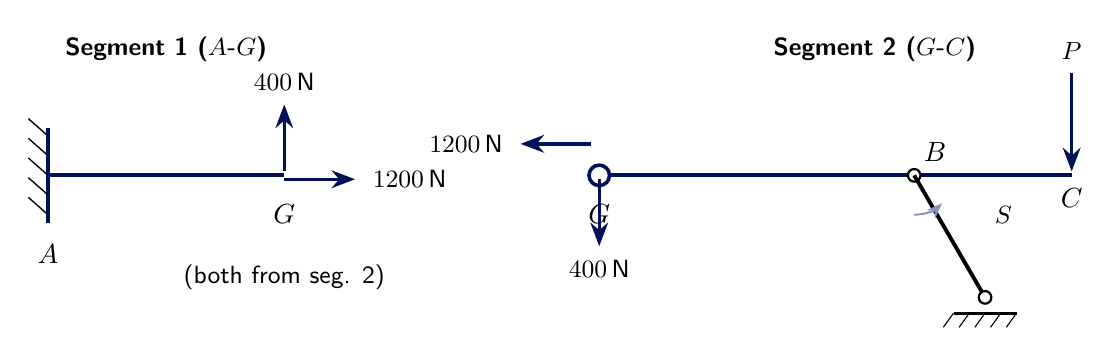
\begin{tikzpicture}
\node[align=center] at (1.5,1.6) {\small \textbf{Segment 1 ($A$-$G$)}};
\einspannung{(0,0)}
\draw[mainblue, line width=1.5pt] (0,0) -- (3,0);
\node[below] at (0,-0.75) {$A$};
\node[below] at (3,-0.25) {$G$};
\draw[force] (3,0.05) -- (3,0.9);
\node[above] at (3,0.95) {\small $400\,\text{N}$};
\draw[force] (3,-0.05) -- (3.9,-0.05);
\node[right] at (4.0,-0.05) {\small $1200\,\text{N}$};
\node[align=center] at (3,-1.3) {\small (both from seg. 2)};
%
\node[align=center] at (10.5,1.6) {\small \textbf{Segment 2 ($G$-$C$)}};
\draw[mainblue, line width=1.5pt] (7,0) -- (13,0);
\gelenk{(7,0)}
\pendelstuetze{(11,0)}
\node[below] at (7,-0.25) {$G$};
\node[above right] at (11,0.05) {$B$};
\node[below] at (13,-0.05) {$C$};
\draw[force] (7,-0.05) -- (7,-0.9);
\node[below] at (7,-0.95) {\small $400\,\text{N}$};
\draw[force] (6.9,0.4) -- (6.0,0.4);
\node[left] at (5.9,0.4) {\small $1200\,\text{N}$};
\draw[force] (13,1.3) -- (13,0.05);
\node[above] at (13,1.35) {\small $P$};
\draw[dim] (11,-0.5) arc (270:315:0.5);
\node[right] at (11.9,-0.5) {\small $S$};
\end{tikzpicture}

% ================= Ex 8.2 problem: fixed + hinge + roller + hinge + roller + overhang =================
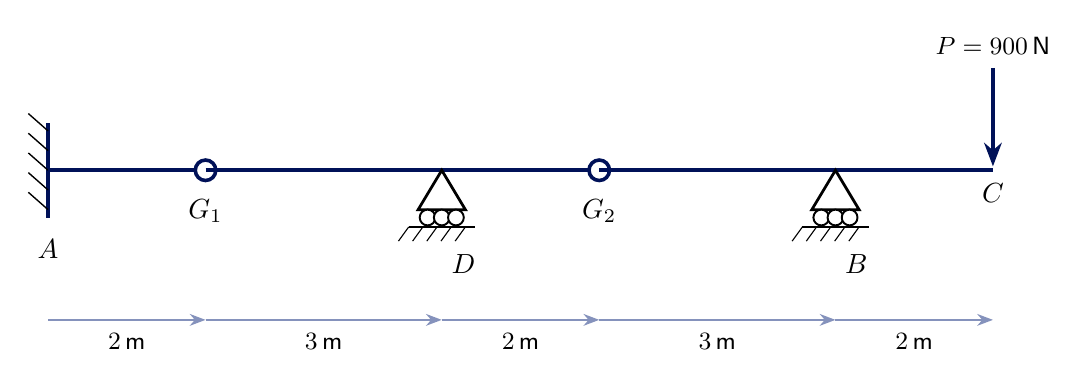
\begin{tikzpicture}
\einspannung{(0,0)}
\draw[mainblue, line width=1.5pt] (0,0) -- (2,0);
\gelenk{(2,0)}
\draw[mainblue, line width=1.5pt] (2,0) -- (7,0);
\loslager{(5,0)}
\gelenk{(7,0)}
\draw[mainblue, line width=1.5pt] (7,0) -- (12,0);
\loslager{(10,0)}
\node[below] at (0,-0.75) {$A$};
\node[below] at (2,-0.25) {$G_1$};
\node[below right] at (5,-0.95) {$D$};
\node[below] at (7,-0.25) {$G_2$};
\node[below right] at (10,-0.95) {$B$};
\node[below] at (12,-0.05) {$C$};
\draw[force] (12,1.3) -- (12,0.05);
\node[above] at (12,1.35) {\small $P=900\,\text{N}$};
\draw[dim] (0,-1.9) -- (2,-1.9);
\node[below] at (1,-1.95) {\small $2\,\text{m}$};
\draw[dim] (2,-1.9) -- (5,-1.9);
\node[below] at (3.5,-1.95) {\small $3\,\text{m}$};
\draw[dim] (5,-1.9) -- (7,-1.9);
\node[below] at (6,-1.95) {\small $2\,\text{m}$};
\draw[dim] (7,-1.9) -- (10,-1.9);
\node[below] at (8.5,-1.95) {\small $3\,\text{m}$};
\draw[dim] (10,-1.9) -- (12,-1.9);
\node[below] at (11,-1.95) {\small $2\,\text{m}$};
\end{tikzpicture}

% ================= Ex 8.2 split free bodies: three segments =================
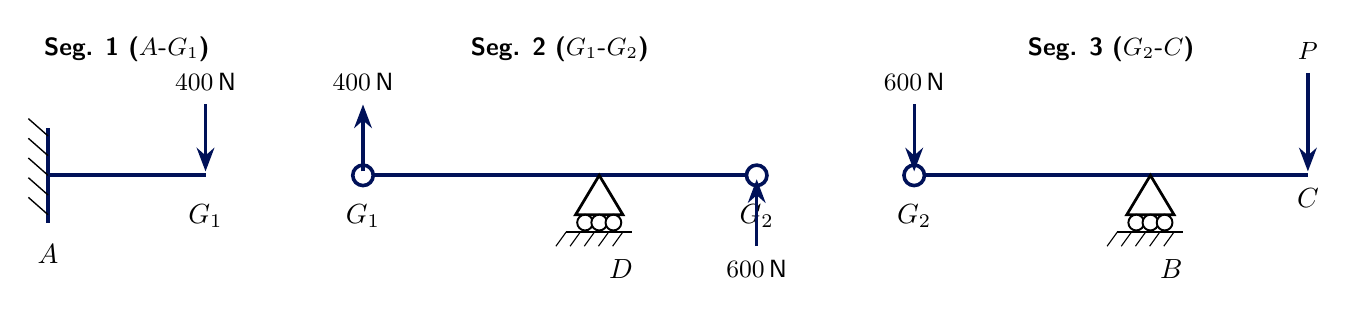
\begin{tikzpicture}
\node[align=center] at (1,1.6) {\small \textbf{Seg. 1 ($A$-$G_1$)}};
\einspannung{(0,0)}
\draw[mainblue, line width=1.5pt] (0,0) -- (2,0);
\node[below] at (0,-0.75) {$A$};
\node[below] at (2,-0.25) {$G_1$};
\draw[force] (2,0.9) -- (2,0.05);
\node[above] at (2,0.95) {\small $400\,\text{N}$};
%
\node[align=center] at (6.5,1.6) {\small \textbf{Seg. 2 ($G_1$-$G_2$)}};
\draw[mainblue, line width=1.5pt] (4,0) -- (9,0);
\gelenk{(4,0)}
\loslager{(7,0)}
\gelenk{(9,0)}
\node[below] at (4,-0.25) {$G_1$};
\node[below right] at (7,-0.95) {$D$};
\node[below] at (9,-0.25) {$G_2$};
\draw[force] (4,0.05) -- (4,0.9);
\node[above] at (4,0.95) {\small $400\,\text{N}$};
\draw[force] (9,-0.9) -- (9,-0.05);
\node[below] at (9,-0.95) {\small $600\,\text{N}$};
%
\node[align=center] at (13.5,1.6) {\small \textbf{Seg. 3 ($G_2$-$C$)}};
\draw[mainblue, line width=1.5pt] (11,0) -- (16,0);
\gelenk{(11,0)}
\loslager{(14,0)}
\node[below] at (11,-0.25) {$G_2$};
\node[below right] at (14,-0.95) {$B$};
\node[below] at (16,-0.05) {$C$};
\draw[force] (11,0.9) -- (11,0.05);
\node[above] at (11,0.95) {\small $600\,\text{N}$};
\draw[force] (16,1.3) -- (16,0.05);
\node[above] at (16,1.35) {\small $P$};
\end{tikzpicture}

% ================= Ex 8.3 problem: fixed + hinge + roller + applied end couple =================
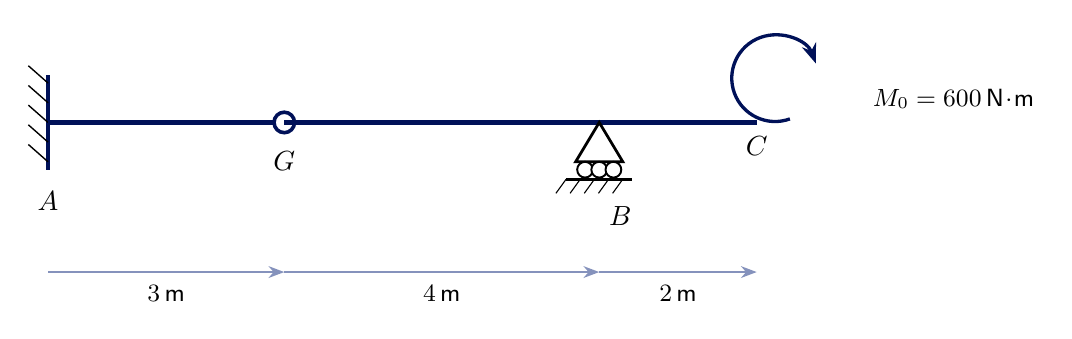
\begin{tikzpicture}
\einspannung{(0,0)}
\draw[mainblue, line width=1.5pt] (0,0) -- (3,0);
\gelenk{(3,0)}
\draw[mainblue, line width=1.5pt] (3,0) -- (9,0);
\loslager{(7,0)}
\node[below] at (0,-0.75) {$A$};
\node[below] at (3,-0.25) {$G$};
\node[below right] at (7,-0.95) {$B$};
\node[below] at (9,-0.05) {$C$};
\draw[moment, {Stealth[length=2.5mm]}-] (9.75,0.75) arc (20:290:0.55);
\node[right] at (10.35,0.3) {\small $M_0=600\,\text{N}\!\cdot\!\text{m}$};
\draw[dim] (0,-1.9) -- (3,-1.9);
\node[below] at (1.5,-1.95) {\small $3\,\text{m}$};
\draw[dim] (3,-1.9) -- (7,-1.9);
\node[below] at (5,-1.95) {\small $4\,\text{m}$};
\draw[dim] (7,-1.9) -- (9,-1.9);
\node[below] at (8,-1.95) {\small $2\,\text{m}$};
\end{tikzpicture}

% ================= Ex 8.3 split free bodies =================
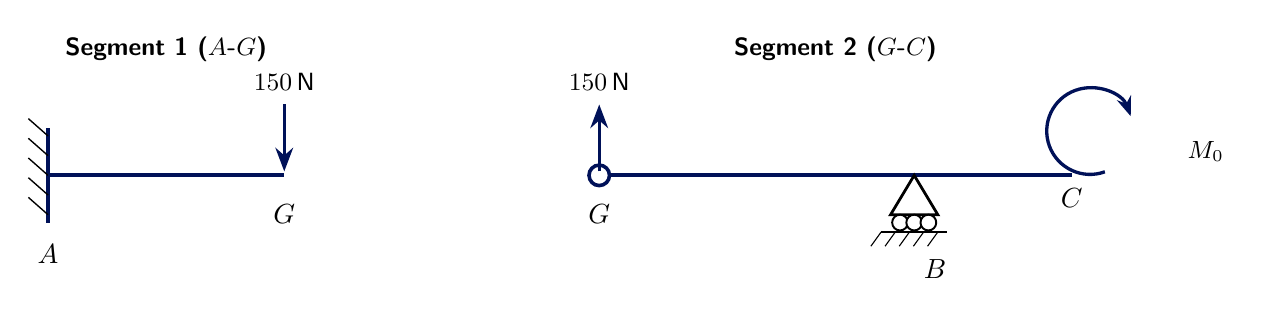
\begin{tikzpicture}
\node[align=center] at (1.5,1.6) {\small \textbf{Segment 1 ($A$-$G$)}};
\einspannung{(0,0)}
\draw[mainblue, line width=1.5pt] (0,0) -- (3,0);
\node[below] at (0,-0.75) {$A$};
\node[below] at (3,-0.25) {$G$};
\draw[force] (3,0.9) -- (3,0.05);
\node[above] at (3,0.95) {\small $150\,\text{N}$};
%
\node[align=center] at (10,1.6) {\small \textbf{Segment 2 ($G$-$C$)}};
\draw[mainblue, line width=1.5pt] (7,0) -- (13,0);
\gelenk{(7,0)}
\loslager{(11,0)}
\node[below] at (7,-0.25) {$G$};
\node[below right] at (11,-0.95) {$B$};
\node[below] at (13,-0.05) {$C$};
\draw[force] (7,0.05) -- (7,0.9);
\node[above] at (7,0.95) {\small $150\,\text{N}$};
\draw[moment, {Stealth[length=2.5mm]}-] (13.75,0.75) arc (20:290:0.55);
\node[right] at (14.35,0.3) {\small $M_0$};
\end{tikzpicture}

\end{document}
